
\section{Konvolučné neurónové siete}
\label{sec:architekuraCNN}

\subsection{Nastavenie parametrov}
\label{subsec:nastavenieparametrov}
Ako bolo spomínané v~kapitole \ref{subsec:convolutionalneuralnetwork} je niekoľko parametrov, ktoré je potrebné
    nastaviť v~konvolučných a pooling vrstvách.
Pre správne fungovanie siete je potrebné nastaviť aj správne hodnoty týchto parametrov, preto v~navrhovaných architektúrach budú
    hodnoty parametrov nastavené na tie najpoužívanejšie.

Veľkosť výstupu a správnosť nastavenia parametrov v~konvolučnej vrstve je možné výpočítať pomocou vzťahu:
\begin{equation}
    \frac{(W - F + 2*P)}{S} + 1
\end{equation}
Kde $W$ je veľkosť vstupných dát, $F$ je veľkosť filtra, $P$ je nastavenie zarovnania, v~prípade nulového zarovnania je hodnota 1 a $S$ je veľkosť kroku.
Pre správné nastavenie musí byť výsledná hodnota celé číslo, kde táto výsledná hodnota udáva aj veľkosť výstupu.
Najpoužívanejšie hodnoty parametrov sú: $F = 3, S = 1, P = 1$ a vstup $W$ o~hodnote, ktorá je deliteľná číslom 2 \cite{odkaz:CNNArchitecture}.

Funkciou pooling vrstvy je znižovanie dimenzionality a zároveň ponechanie dôležitých informácií, ako najpoužívanejšie hodnoty parametrov sú
    veľkosť filtra 2x2 s~krokom 2 pri použití MaxPooling vrstvy \cite{odkaz:CNNArchitecture}.

% TODO batch-size, epochy
% CNN sa trenuje v cykloch nazyvanych epochy, v kazdej epoche prejdu cez sieť vsetky obrazky na ktorych sa sieť uci,
% pre ucenie je potrebne zvolit vhodny pocet tychro epoch aby sieť podala najelpsie vysledky a zaroven sa nepretrenovala.
% Preto je vhodne ukoncit trenovanie v bode kedy klesa presnosť siete na validacnych datach, v takom pripade to moze vies k pretrénovaniu siete
% na trenovacich datach.

\subsection{Návrh architektúr}
\label{subsec:navrharchitektur}
Prvý model siete je inšpirovaný architektúrou AlexNet (viď. \ref{subsec:popularCNN}).
Model obsahuje celkovo 15 vrstiev, z~ktorých 4 je konvolučných, 4 max pooling, 5 dropout a 2 dense vrstvy.
Veľkosť vstupných dát do prvej vrstvy je 128x128x3.
Vo všetkých konvolučných vrstvách sú použité filtre o~veľkosti 3x3 s~krokom 1 a použitím nulového zarovnania.

V~modeli sa každou konvolučnou vrstvou zdvojnásobuje počet filtrov, z~počiatočných 16 až na 128 v~poslednej vrstve.
Pooling vrstvy sú typu max, veľkosť filtra je 2x2 s~posunom 2 po každej osi.
Za každou pooling vrstvou sa nachádza Droupout vrstva s~nastavením 0.2, čiže 20 percent náhodných prepojení sa ignoruje.

Po štyroch blokoch konvolučnej, pooling a droupout vrstvy nasleduje dense vrstva s~počtom prepojení 1024 a dropout vrstva s~nastavním 0.5.
Ako posledná je dense vrstva s~2 alebo 72 prepojeniami a softmax klasifikátorom, počet výstupov závísí od toho, či určujeme typ alebo náklon zbrane.
V~celej sietí sú použité ReLu aktivačné funkcie.

\begin{figure}[H]
    \centering
    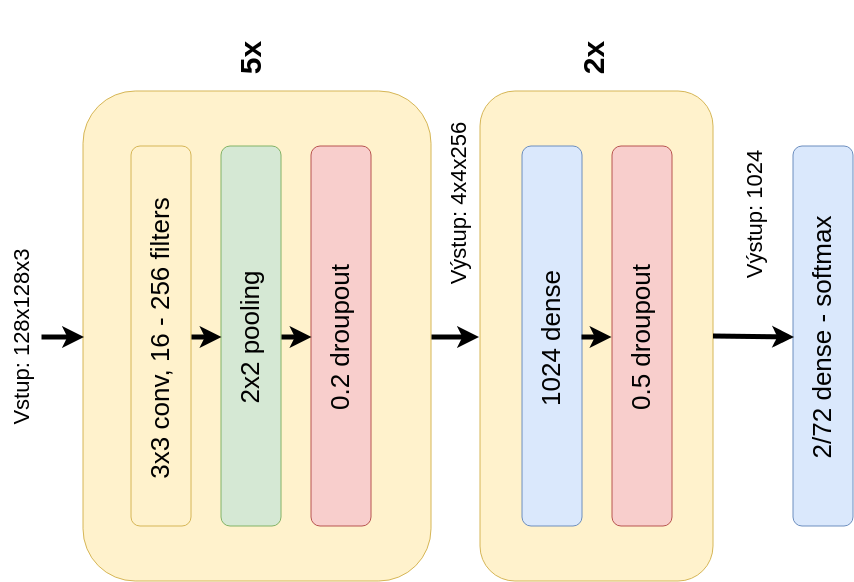
\includegraphics[width=0.6\textwidth]{AlexNet_Like}
    \caption{AlexNet-Like navrhovaná architektúra.}
    \label{pic:kNN}
\end{figure}

% ----------- DRUHY NAVRH -----------

Druhý navrhovaný model je inšpirovaný architektúrou VGG sietí (viď. \ref{subsec:popularCNN}).
Vzhľadom na možnosti výkonu na ktorom bude trénovanie prebiehať, je navrhovaná sieť o~dva bloky vrstviev menšia a taktiež konvolučne vrstvy obsahujú menej filtrov.

Celkovo sieť obsahuje 2 bloky obsahujúce 2 konvolučné vrstvy s~počtom filtrov 32 a 64, pooling a droupout vrstvu s~20\% ignorovaním prepojení.
Ďalej nasledujú 3 konvolučné vrstvy so 128 filtrami a pooling vrstva.
Ako posledné sú 2 bloky obsahujúce dense vrstvu s~počtom prepojení 2048 a dropout vrstvu s~ignorovaním nastaveným na 50\%.
Posledná výstupná vrstva obsahuje 2 alebo 72 prepojení so softmax klasfikátorom.
Každá konvolučná vrstva obsahuje filtre o~veľkosti 3x3, krokom 1 a s~použitím nulového doplnku.
Pooling vrstvy sú typu max, veľkosť filtra je 2x2 s~posunom 2 po každej osi.
V~celej sietí je použitá ReLu aktivačná funkcia.

\begin{figure}[H]
    \centering
    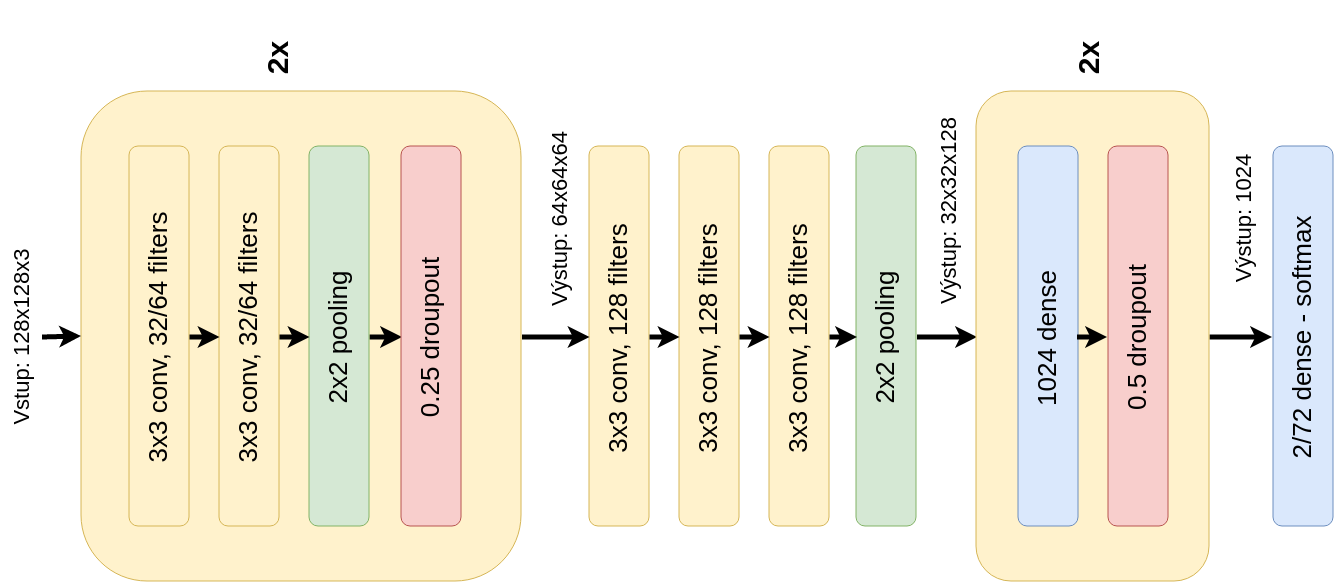
\includegraphics[width=0.8\textwidth]{VGG_Like}
    \caption{VGG-Like navrhovaná architektúra.}
    \label{pic:kNN}
\end{figure}

\subsection{Hodnotenie presnosti modelov}
\label{subsec:hodnoteniepresnosti}
Hodnotenie presnosti modelov bude prebiehať pomocou dvoch metrík.

Prvá z~metrík je tzv. chybová alebo tiež kontigenčná matica.
Každý stĺpec v~matici predstavuje klasifikované triedy a jednotlivé riadky predstavujú správne triedy.
Tabuľka \ref{tab:chybovamatica} zobrazuje túto maticu.
Hodnota TP označuje počet správne klasifikovaných obrázkov triedy true, hodnota FP označuje počet nesprávne klasfikovaných obrázkov triedy true.
Hodnota TN označuje počet správne klasifikovaných obrázkov triedy false, hodnota FN označuje počet nesprávne klasifikovaných obrázkov triedy false \cite{odkaz:ChybovaMatica}.
\begin{table}[H]
    \centering
    \label{tab:chybovamatica}
        \begin{tabular}{lllc}
                                                                &                                   & \multicolumn{2}{c}{Klasifikované hodnoty}                                           \\ \cline{3-4} 
                                                                & \multicolumn{1}{l|}{}             & \multicolumn{1}{c|}{Trieda false}        & \multicolumn{1}{c|}{Trieda true}         \\ \cline{2-4} 
        \multicolumn{1}{c|}{\multirow{2}{*}{Správne hodnoty}} & \multicolumn{1}{c|}{Trieda false} & \multicolumn{1}{l|}{TN (True Negative)}  & \multicolumn{1}{c|}{FP (False Positive)} \\ \cline{2-4} 
        \multicolumn{1}{c|}{}                                 & \multicolumn{1}{c|}{Trieda true}  & \multicolumn{1}{l|}{FN (False Negative)} & \multicolumn{1}{c|}{TP (True Positive)}  \\ \cline{2-4} 
    \end{tabular}
    \caption{Chybová matica}
\end{table}
Pre prípad tejto práce si môžeme previesť triedu true na triedu krátke zbrane a triedu false na triedu dlhé zbrane.
Ako hodnotenie presnosti bude použitá metrika úspešnosť (angl. \textit{Accuracy}).

Úspešnosť - táto hodnota určuje ako často klasfikátor správne klasifikoval daný obrázok, počíta sa ako:
\begin{equation}
    Accuracy = \frac{TP + TN}{TP + TN + FP + FN}
\end{equation}

Ako druhá metrika, pre určenie presnosti modelov ktoré určujú náklon zbrane, bude implementovaná funkcia \textit{angle\_error}, ako bolo opísané v~\ref{subsec:odchylkachyby}.
Hodnotenie funguje tak, že je nastavená prahová hodnota uhla podľa ktorej sa určuje, či daná predpoveď siete bola správna alebo nie.
Správne určenie je vypočítané, ako rozdiel medzi skutočným uhlom a predpovedaným uhol pomocou natrenovaného modelu, ak je rozdiel menší ako prahová hodnota, tak predikcia
    sa považuje za správnu v~opačnom prípade za nesprávnu.
